\addcontentsline{toc}{chapter}{Занятие 5. Условные вероятности. Независимость}
\chapter*{Занятие 5. Условные вероятности. Независимость}

\addcontentsline{toc}{section}{Контрольные вопросы и задания}
\section*{Контрольные вопросы и задания}

\subsubsection*{Какие события называются независимыми?}

$A$ и $B$ --- независимы, если $P \left( A \cap B \right) = P \left( A \right) P \left( B \right) $.

\subsubsection*{Какие события называются несовместимыми?}

В теории вероятностей несколько событий называются несовместными, или несовместимыми, если никакие из них не могут появиться одновременно в результате однократного проведения эксперимента (опыта).

\subsubsection*{Запишите формулу для вычисления условной вероятности.}

Условная вероятность события $A$ при условии, что событие $B$ произошло --- это выражение
$$P \left( A/B \right) =
\frac{P \left( A \cap B \right) }{P \left( B \right) }.$$

\addcontentsline{toc}{section}{Домашнее задание}
\section*{Домашнее задание}

\subsubsection*{5.15}

\textit{Задание.} Из колоды игральных карт наугад вынута одна карта.
Найдите вероятность того, что:
\begin{enumerate}[label=\alph*)]
\item эта карта является красной масти, при условии, что она является красной;
\item порядок карты является выше чем 10, если известно что она красной масти;
\item эта карта является тузом, если известно, что она является красной.
\end{enumerate}

\textit{Решение.} 
\begin{enumerate}[label=\alph*)]
\item нужно найти вероятность события $A$ при условии выполнения события $B$.
Опишем оба события.
Событие $А =$ \{вынята карта красной масти\}.
Красных карт половина от всего количества.
Событие $B =$ \{карта является красной\}.
Видим, что события $A$ и $B$ идентичны, поэтому $P \left( A \cap B \right) = P \left( A \right) = P \left( B \right)$.
Тогда условная вероятность события равна
$$P \left( A/B \right) =
\frac{P \left( A \cap B \right)}{P \left( B \right) } =
\frac{ \frac{1}{2} }{ \frac{1}{2} } =
1;$$
\item нужно найти вероятность события $A$ при условии выполнения события $B$.
Опишем оба события.
Событие $А =$ \{порядок выбранной карты больше десяти\}.
Такими картами является валет, дама, король и туз любой масти.
Событие $B =$ \{карта является красной\}.
Его вероятность равна
$$P \left( B \right) =
\frac{1}{2}.$$
Пересечение событий $A$ и $B$ даёт такие карты как валет, дама, король и туз красных мастей.
Вероятность пересечения равна
$$P \left( A \cap B \right) =
\frac{2 \cdot 4}{52} =
\frac{4}{26} =
\frac{2}{13}.$$
Тогда условная вероятность события равна
$$P \left( A/B \right) =
\frac{P \left( A \cap B \right)}{P \left( B \right) } =
\frac{ \frac{2}{13} }{ \frac{1}{2} } =
\frac{4}{13};$$
\item нужно найти вероятность события $A$ при условии выполнения события $B$.
Опишем оба события.
Событие $А =$ \{карта является тузом\}.
Такими картами являются 4 туза.
Событие $B =$ \{карта является красной\}.
Его вероятность равна
$$P \left( B \right) =
\frac{1}{2}.$$
Пересечение событий $A$ и $B$ даёт два красных туза.
Вероятность пересечения равна
$$P \left( A \cap B \right) =
\frac{2}{52} =
\frac{1}{26}.$$
Тогда условная вероятность события равна
$$P \left( A/B \right) =
\frac{P \left( A \cap B \right)}{P \left( B \right) } =
\frac{ \frac{1}{26} }{ \frac{1}{2} } =
\frac{2}{26} =
\frac{1}{13}.$$
\end{enumerate}

\subsubsection*{5.16}

\textit{Задание.} Игральный кубик подбросили дважды.
Найдите вероятность того, что сумма очков является больше 7, если известно, что:

\begin{enumerate}[label=\alph*)]
\item при первом подбрасывании быпало одно очко;
\item при первом подбрасывании выпало меньше, чем 5 очков.
\end{enumerate}

\textit{Решение.}
Вероятностное пространство эксперимента,
которое состоит в подбрасывании игрального кубика дважды,
опишем множеством
$ \Omega =
\left\{ \left( x, y \right), \, x = \overline{1, 6}, \, y = \overline{1, 6} \right\} $,
где через $x$ обозначим количество очков,
которые выпали при первом подбрасывании игрального кубика, а через $y$ --- количество очков, которые выпали при втором его подбрасывании.
Нам нужно вычислить вероятность $P \left( \left. x+y>7 \right| x=1 \right) $ и $P \left( \left. x+y>7 \right| x<5 \right) $.
По определению вероятности:
$$P \left( \left. x+y>7 \right| x=1 \right) =
\frac{P \left( x+y>7, \, x=1 \right) }{P \left( x=1 \right) }.$$
Поскольку
$ \left\{ \left( x, y \right) \in \Omega: \, x + y > 7, \, x = 1 \right\} =
\varnothing $,
а $ \left\{ \left( x, y \right) \in \Omega: \, x = 1 \right\} =  \\ = \left\{ \left( 1, y \right), \, y = \overline{1, 6} \right\} $, то
$$P \left( \left. x+y>7 \right| x=1 \right) =
\frac{ \varnothing }{ \frac{6}{36} } =
\varnothing.$$
Далее
$$P \left( \left. x+y>7 \right| x<5 \right) =
\frac{P \left( \left. x+y>7 \right| x<5 \right) }{P \left( x<5 \right) }.$$
Понятно, что
$$P \left( x<5 \right) =
\frac{4}{6} =
\frac{2}{3}.$$
А для вероятности в числителе имеем:
\begin{equation*}
\begin{split}
P \left( \left. x+y>7 \right| x<5 \right) =
\sum \limits_{k=1}^4 P \left(x=k, \, k+y>7 \right) = \\
= \sum \limits_{k=1}^4 P \left( x=k \right) P \left( y>7-k \right) =
P \left( x=1 \right) P \left( y>6 \right) +
P \left( x=2 \right) P \left( y>5 \right) + \\
+ P \left( x=3 \right) \left( y>4 \right) +
P \left( x=4 \right) P \left( y>3 \right) =
\frac{1}{6} \left(\varnothing +\frac{1}{6} + \frac{2}{6} + \frac{3}{6} \right) =
\frac{1}{6} \cdot \frac{6}{6} = \\
= \frac{6}{36} =
\frac{1}{6}.
\end{split}
\end{equation*}

Тут мы воспользовались тем, что результаты первого и второго подбрасываний являются независимыми событиями.
Таким образом:
$$P \left( \left. x+y>7 \right| x<5 \right) =
\frac{P \left( x+y>5, \, x<5 \right) }{P \left( x<5 \right) } =
\frac{ \frac{1}{6} }{ \frac{2}{3} } =
\frac{1}{4}.$$

\subsubsection*{5.17}

\textit{Задание.} Дважды подброшена монета.
Рассмотрим следующие события:
$A =$ \{при первом подбрасывании выпала решка\}, $B =$ \{при втором подбрасывании выпала решка\}, $C =$ \{результат обеих подбрасываний одинаковый\}.
Покажите, что события $A, \, B, \, C$ попарно независимы, но не независыми в совокупности.

\textit{Решение.} События $A_i$ и $A_j$ называются попарно независимыми, если для $ \forall i \neq j \rightarrow A_i $ и $A_j$ --- независимы.

Пространством элементарных исходов является множество векторов
$ \Omega = \\
= \left\{ \left( i, j \right), \, i, j \in \left\{ 0, 1 \right\} \right\}$,
где $0$ означает, что выпал герб, $1$ --- выпала решка, $i$ --- результат первого подбрасывания, $j$ --- результат второго подбрасывания.
Пространство элементарных событий содержит $ \left| \Omega \right| = 2^2 = 4$ элемента.

Опишем данные события.
Событие $A = \left\{ \left( 1, 0 \right), \, \left( 1, 1 \right) \right\} $.
Вероятность выпадения при первом подбрасывании решки равна
$$P \left( A \right) =
\frac{2}{4} =
\frac{1}{2}.$$

Опишем событие $B = \left\{ \left( 0, 1 \right), \, \left( 1, 1 \right) \right\} $.
Вероятность выпадения решки при втором подбрасывании равна
$$P \left( B \right) =
\frac{2}{4} =
\frac{1}{2}.$$

Опишем событие $C = \left\{ \left( 0, 0 \right), \, \left( 1, 1 \right) \right\} $.
Вероятность того, что результат двух подбрасываний будет одинаковым, равна
$$P \left( C \right) =
\frac{2}{4} =
\frac{1}{2}.$$

Найдём вероятности пересечения событий $A$ и $B$:
$$P \left( A \cap B \right) =
P \left( \left\{ \left( 1, 1 \right) \right\} \right) =
\frac{1}{4}.$$
Найдём произведение вероятностей этих событий:
$$P \left( A \right) P \left( B \right) =
\frac{1}{2} \cdot \frac{1}{2} =
\frac{1}{4}.$$
Получаем, что $P \left( A \cap B \right) = P \left( A \right) P \left( B \right) $, значит эти события независимы.

Найдём вероятности пересечения событий $A$ и $C$:
$$P \left( A \cap C \right) =
P \left( \left\{ \left( 1, 1 \right) \right\} \right) =
\frac{1}{4}.$$
Найдём произведение вероятностей этих событий:
$$P \left( A \right) P \left( C \right) =
\frac{1}{2} \cdot \frac{1}{2} =
\frac{1}{4}.$$
Получаем, что $P \left( A \cap C \right) = P \left( A \right) P \left( C \right) $, значит эти события независимы.

Найдём вероятности пересечения событий $B$ и $C$:
$$P \left( B \cap C \right) =
P \left( \left\{ \left( 1, 1 \right) \right\} \right) =
\frac{1}{4}.$$
Найдём произведение вероятностей этих событий:
$$P \left( B \right) P \left( C \right) =
\frac{1}{2} \cdot \frac{1}{2} =
\frac{1}{4}.$$
Получаем, что $P \left( B \cap C \right) = P \left( B \right) P \left( C \right) $, значит эти события независимы.

События $A, \, B, \, C$ называются независимыми в совокупности, если имеет место равенство:
$P \left( A \cap B \cap C \right) =
P \left( A \right) P \left( B \right) P \left( C \right) $.

Проверим это равенство для данной задачи:
$$P \left( A \cap B \cap C \right) =
P \left( \left\{ \left( 1, 1 \right) \right\} \right) =
\frac{1}{4}.$$
Найдём произведение вероятностей всех трёх событий:
$$P \left( A \right) P \left( B \right) P \left( C \right) =
\frac{1}{2} \cdot \frac{1}{2} \cdot \frac{1} {2} =
\frac{1}{8}.$$
Получили, что равенство не выполняется, поэтому события не независимы.

\subsubsection*{5.18}

\textit{Задание.} В урне $7$ белых и $3$ чёрных шарика.
Из неё наугад вынимают три шарика.
Известно, что среди них есть чёрный шарик.
Найдите вероятность того, что два других шарика белые.

\textit{Решение.}
Пространство элементарных событий имеет вид
$ \Omega = \\ = \left\{ \left( i, j, k \right): i, k, k \in \right.$ \{белый, чёрный\}, где $i, j, k$ --- цвета вытянутых шариков.
Выпишем все его элементы: $ \Omega = $ \{(чёрный, чёрный, чёрный), (чёрный, белый, белый), (белый, чёрный, белый), (белый, белый, чёрный),
(чёрный, чёрный, белый), (чёрный, белый, белый), (белый, чёрный, чёрный), (белый, белый, белый)\}.
Видим, что $ \left| \Omega \right| = 2^3 = 8$.

Событие $B =$ \{среди выбранных шаров есть чёрный шар\} = \{(чёрный, чёрный, чёрный),
(чёрный, белый, белый), (белый, чёрный, белый), (белый, белый, чёрный),
(чёрный, чёрный, белый), (чёрный, белый, чёрный), (белый, чёрный, чёрный)\}.
Вероятность этого события равна
$$P \left( B \right) =
\frac{ \left| B \right| }{ \left| \Omega \right| } =
\frac{7}{8}.$$

Опишем событие $A =$ \{два шара белые\} = \{(чёрный, белый, белый)\}.

Найдём вероятность пересечения событий $A$ и $B: \, P \left( A \cap B \right) =$ \{(чёрный, белый, белый)\}.

Тогда условная вероятность события $A$ при условии, что $B$ произошло равна
$$P \left( A/B \right) =
\frac{P \left( A \cap B \right) }{P \left( B \right) } =
\frac{ \frac{1}{8} }{ \frac{7}{8} } =
\frac{1}{7}.$$

\subsubsection*{5.19}

\textit{Задание.} Точка $ \xi = \left( \xi_1, \xi_2 \right) $ наугад выбрана в квадрате $ \left[ 0, 1 \right]^2$.
Пусть $B = \left\{ \xi_1 + \xi_2 \leq 1 \right\} $.
Вычислите условную вероятность $P \left( \left. A \right| B \right) $, если:
\begin{enumerate}[label=\alph*)]
\item $A = \left\{ \left| \xi_1 + \xi_2 \right| < 1 \right\} $;
\item $A = \left\{ \xi_1 \cdot \xi_2 < 1/2 \right\} $;
\item $A = \left\{ \max \left\{ \xi_1, \xi_2 \right\} < 1/2 \right\} $;
\item $A = \left\{ \xi_1^2 + \xi_2^2 < 1/4 \right\} $;
\item $A = \left\{ \xi_1 > \xi_2 \right\} $.
\end{enumerate}

\textit{Решение.}
Вероятностное пространство эксперимента,
которое состоит в выборе точки в квадрате
$ \left[ 0, 1 \right]^2$, опишем множеством
$$ \Omega =
\left\{ \left( \xi_1, \xi_2 \right), \,
0 \leq \xi_1 \leq 1, \,
0 \leq \xi_2 \leq 1 \right\},$$
где через $ \xi_1$ обозначена первая координата точки, а через $ \xi_2$ --- вторая координата.

Вычислим вероятность события $B$.
Это прямоугольный равнобедренный треугольник с катетами длиной $1$.
Тогда площадь этой фигуры равна
$$S_B =
\frac{1}{2} \cdot 1 \cdot 1 =
\frac{1}{2}.$$

\begin{enumerate}[label=\alph*)]
\item Событие $A$ --- это прямоугольный равнобедренный треугольник с катетами длиной $1$.
Вероятность пересечения событий $A$ и $B$ равна
$$P \left( A \cap B \right) =
\frac{1}{2}.$$
Тогда условная вероятность равна
$$P \left( \left. A \right| B \right) =
\frac{P \left( A \cap B \right) }{P \left( B \right) } =
\frac{ \frac{1}{2} }{ \frac{1}{2} } =
1;$$
\item событие $A$ --- это часть квадрата под веткой гиперболы
$$ \xi_2 = \frac{1}{2 \xi_1}.$$
Вероятность пересечения событий $A$ и $B$ равна
$$P \left( A \cap B \right) =
\frac{1}{2}.$$
Тогда условная вероятность равна
$$P \left( \left. A \right| B \right) =
\frac{P \left( A \cap B \right) }{P \left( B \right) } =
\frac{ \frac{1}{2} }{ \frac{1}{2} } =
1;$$
\item множество $A$ --- это фигура,
образованная вырезанием из квадрата со сторонами длиной $1$ квадрат со сторонами длиной $1/2$ (рис. \ref{fig:517}).
\begin{figure}[h!]
  \centering
  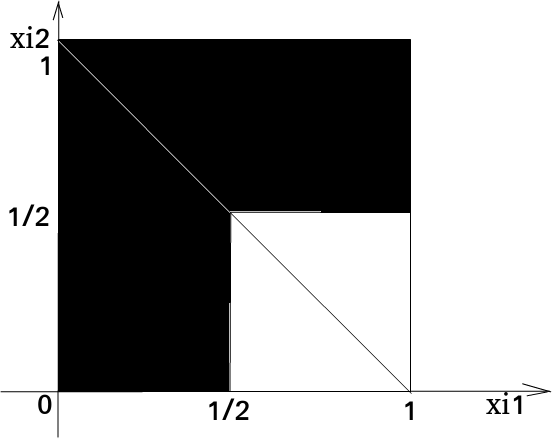
\includegraphics[width=.4\textwidth]{./pictures/5_17.png}
  \caption{Точки множества $A$}
  \label{fig:517}
\end{figure}
Вероятность пересечения событий $A$ и $B$ равна
$$P \left( A \cap B \right) =
\frac{1}{2} \left[ \cdot 1^2 - \left( \frac{1}{2} \right)^2 \right] =
\frac{1}{2} \cdot \frac{3}{4} =
\frac{3}{8}.$$
Тогда условная вероятность равна
$$P \left( \left. A \right| B \right) =
\frac{P \left( A \cap B \right) }{P \left( B \right) } =
\frac{ \frac{3}{8} }{ \frac{1}{2} } =
\frac{3}{4};$$
\item множество $A$ --- четвёртая часть круга с радиусом $1/2$.
Вероятность пересечения событий $A$ и $B$ равна
$$P \left( A \cap B \right) =
\frac{1}{4} \cdot \pi \left( \frac{1}{2} \right)^2 =
\frac{ \pi }{16}.$$
Тогда условная вероятность равна
$$P \left( \left. A \right| B \right) =
\frac{P \left( A \cap B \right) }{P \left( B \right) } =
\frac{ \frac{ \pi }{16} }{ \frac{1}{2} } =
\frac{ \pi }{8};$$
\item множество $A$ --- это равнобедренный прямоугольный треугольник с катетами длиной $1$.
Вероятность пересечения событий $A$ и $B$ равна
$$P \left( A \cap B \right) =
\frac{1}{4} \cdot 1^2 =
\frac{1}{4}.$$
Тогда условная вероятность равна
$$P \left( \left. A \right| B \right) =
\frac{P \left( A \cap B \right) }{P \left( B \right) } =
\frac{ \frac{1}{4} }{ \frac{1}{2} } =
\frac{1}{2}.$$
\end{enumerate}

\subsubsection*{5.20}

\textit{Задание.} Монета, для которой вероятность выпадения решки равна $p$, подбрасывается $n$ раз.
Пусть событие $A$ состоит в том, что решка выпала при первом подбрасывании, а событие $B_k$ --- в том, что выпало ровно $k$ решек.
Для каких пар $ \left( n, k \right) $ события $A$ и $B_k$ являются независимыми?

\textit{Решение.}
Опишем вероятностное пространство
$ \Omega = \\
= \left\{ \left( x_1, x_2, \dotsc, x_n \right), \,
x_i \in \left\{ 0, 1\right\}, \,
i = \overline{1, n} \right\} $,
где 1 означает, что выпала решка, 0 --- выпал орёл.
На каждом месте может стоять либо единица, либо ноль.
Поэтому $ \left| \Omega \right| =2^n$.

Опишем событие $A = \left\{ \left( x_1, x_2, \dotsc, x_n \right) \in \Omega, \, x_1 = 1 \right\} $.
На первом месте может стоять только единица.
Количество способов её выбрать равна одному.
Тогда остаётся посчитать, сколько есть вариантов выпадения монеты при остальных $n - 1$ подбрасывании.
Имеем $ \left| A \right| = 2^{n-1} p \cdot \sum \limits_{i=1}^{n-1} \left( 1-p \right)^i p^{n-i}$.
Тогда вероятность события $A$ равна
$$P \left( A \right) =
\frac{2^{n-1} p \cdot \sum \limits_{i=1}^{n-1} \left( 1-p \right)^i p^{n-i}}{2^n} =
\frac{p \cdot \sum \limits_{i=1}^{n-1} \left( 1-p \right)^i p^{n-i}}{2}.$$

Опишем событие $B_k = \left\{ \left( x_1, x_2, \dotsc, x_n \right) \in \Omega, \, \sum \limits_{i=1}^k x_i = k \right\} $.
На $k$ местах могут стоять только единицы, на остальных $n - k$ местах --- только нули.
Найдём количество способов выбрать $k$ мест, где будут единицы.
Это $C_n^k p^k \left( 1-p \right)^{n-k}$.
Тогда вероятность равна
$$P \left( B_k \right) =
\frac{C_n^k p^k \left( 1-p \right)^{n-k}}{2^n}.$$

Чтобы события были независимы, нужно, чтобы вероятность пересечения этих событий равнялась произведению их вероятностей.
Найдём произведение вероятностей:
\begin{equation*}
\begin{split}
P \left( A \right) P \left( B_k \right) =
\frac{p \cdot \sum \limits_{i=1}^{n-1} \left( 1-p \right)^i p^{n-i}}{2} \cdot \frac{C_n^k p^k \left( 1-p \right)^{n-k}}{2^n} = \\
= \frac{p p^k \left( 1-p \right)^{n-k} C_n^k \cdot \sum \limits_{i=1}^{n-1} p^{n-i} \left( 1-p \right)^i}{2^{n+1}} = \\
= \frac{p^{k+1} \left( 1-p \right)^{n-k} C_n^k \cdot \sum \limits_{i=1}^{n-1} p^{n-i} \left( 1-p \right)^i}{2^{n+1}}.
\end{split}
\end{equation*}

Найдём вероятность переечения этих событий:
$$P \left( A \cap B \right) =
P \left( \left\{ \left( x_1, x_2, \dotsc, x_n \right) \in \Omega, \, \sum \limits_{i=1}^k x_i = k, \, x_1 = 1 \right\} \right).$$
Нужно выбрать $k - 1$ место, где будут единицы.
Тогда
$$P \left( A \cap B \right) =
\frac{p^k \left( 1-p \right)^{n-k} C_n^{k-1}}{2^n}.$$

Приравняем полученные результаты:
$$ \frac{p^{k+1} \left( 1-p \right)^{n-k} C_n^k \cdot \sum \limits_{i=1}^{n-1} p^{n-i} \left( 1-p \right)^i}{2^{n+1}} =
\frac{p^k \left( 1-p \right)^{n-k} C_n^{k-1}}{2^n}.$$
Сократим на
$$\frac{p^k \left( 1-p \right)^{n-k}}{2^n}.$$
Получим:
$$ \frac{p C_n^k \cdot \sum \limits_{i=1}^{n-1} p^{n-i} \left( 1-p \right)^i}{2} =
C_n^{k-1}.$$
Распишем:
$$ \frac{p \cdot \sum \limits_{i=1}^{n-1} p^{n-i} \cdot n!}{2k! \left( n-k \right)!} =
\frac{n!}{ \left( k-1 \right)! \left( n-k+1 \right)!}.$$
Сократим на $n!$ и внесём $p$ под знак суммы:
$$\frac{\sum \limits_{i=1}^{n-1} p^{n-i+1}}{2k! \left( n-k \right)!} = \frac{1}{ \left( k-1 \right)! \left( n-k+1 \right)!}.$$
Распишем факториалы:
$$\frac{\sum \limits_{i=1}^{n-1} p^{n-i+1}}{2 \left( k-1 \right)!k \left( n-k \right)!} = \frac{1}{ \left( k-1 \right)! \left( n-k \right)! \left(n-k+1 \right)!}.$$
Сократим:
$$\frac{\sum \limits_{i=1}^{n-1} p^{n-i+1}}{2k} = \frac{1}{n-k+1}.$$

\subsubsection*{5.21}

\textit{Задание.} Вероятность безотказной работы реле при перегреве равна $0.95$, при вибрации --- $0.9$, при перегреве и вибрации --- $0.8$.
Найдите вероятность отказа реле, если вероятность перегрева равна $0.2$, вероятность вибрации --- $0.1$, и считая, что перегрев и вибрация являются независимыми событиями.

\textit{Решение.}
Пусть событие $A =$ \{реле перегрелось\}, событие $B =$ \{произошла вибрация\}, событие $C =$ \{произошёл отказ реле\}, такие что
\begin{equation*}
\begin{split}
P \left( A \right) = 0.2, \,
P \left( B \right) = 0.1, \,
P \left( \left. \overline{C} \right| A \right) = 0.95, \,
P \left( \left. \overline{C} \right| B \right) = 0.9, \\
P \left( \left. \overline{C} \right| A \cap B \right) = 0.2.
\end{split}
\end{equation*}

Распишем условную вероятность:
$$P \left( \left. \overline{C} \right| A \right) =
\frac{P \left( \overline{C} \cap A \right) }{P \left( A \right) } =
\frac{P \left( \overline{C} \cap A \right) }{0.2} =
0.95.$$
Отсюда $P \left( \overline{C} \cap A \right) = 0.2 \cdot 0.95 = 0.19$.

Распишем условную вероятность:
$$P \left( \left. \overline{C} \right| B \right) =
\frac{P \left( \overline{C} \cap B \right) }{P \left( B \right) } =
\frac{P \left( \overline{C} \cap B \right) }{0.1} =
0.9.$$
Отсюда $P \left( \overline{C} \cap B \right) = 0.1 \cdot 0.9 = 0.09$.

Распишем условную вероятность:
\begin{equation*}
\begin{split}
P \left( \left. \overline{C} \right| A \cap B \right) =
\frac{P \left( \overline{C} \cap A \cap B \right) }{P \left( A \cap B \right) } =
\frac{P \left( \overline{C} \cap A \cap B \right) }{P \left( A \right) P \left( B \right) } =
\frac{P \left( \overline{C} \cap A \cap B \right) }{0.2 \cdot 0.1} = \\
= \frac{P \left( \overline{C} \cap A \cap B \right) }{0.02} =
0.2.
\end{split}
\end{equation*}
Отсюда $P \left( \overline{C} \cap A \cap B \right) = 0.2 \cdot 0.02 = 0.004$.

Посчитаем
$P \left( \overline{ \overline{C} \cap A} \right) =
P \left( C \cup \overline{A} \right) =
P \left( C \right) + P \left( \overline{A} \right) - P \left( C \cap \overline{A} \right) =
P \left( C \right) + \\
+ 1 - 0.2 - P \left( C \cap \overline{A} \right) =
1 - 0.19$.
Тогда $P \left( C \right) - P \left( C \cap \overline{A} \right) = 0.2 - 0.19 = 0.01$.

Найдём
$P \left( \overline{ \overline{C} \cap B} \right) =
P \left( C \cup \overline{B} \right) =
P \left( C \right) + P \left( \overline{B} \right) - P \left( C \cap \overline{B} \right) =
P \left( C \right) + \\ + 1 - 0.1 - P \left( C \cap \overline{B} \right) =
1 - 0.09.$
Отсюда $P \left( C \right) - P \left( C \cap \overline{B} \right) = 0.1 - 0.09 = 0.01$.

Найдём
$P \left( \overline{ \overline{C} \cap A \cap B} \right) =
P \left( C \cup \overline{A} \cup \overline{B} \right) =
P \left( C \right) + P \left( \overline{A} \right) + P \left( \overline{B} \right) - \\
- P \left( C \cap \overline{A} \right) - P \left( C \cap \overline{B} \right) - P \left( \overline{A} \cap \overline{B} \right) +
P \left( C \cap \overline{A} \cap \overline{B} \right) =
P \left( C \right) + 1 - 0.2 + 1 - \\ 
- 0.1 - P \left( C \cap \overline{A} \right) - P \left( C \cap \overline{B} \right) - \left( 1 - 0.2 \right) \left( 1 - 0.1 \right) +
P \left( C \cap \overline{A} \cap \overline{B} \right) =
P \left( C \right) - \\
- P \left( C \cap \overline{A} \right) -
P \left( C \cap \overline{B} \right) +P \left( C \cap \overline{A} \cap \overline{B} \right) + 0.98 =
1 - 0.004 =
0.996$.
Отсюда
$P \left( C \right) -
P \left( C \cap \overline{A} \right) -
P \left( C \cap \overline{B} \right) + P \left( C \cap \overline{A} \cap \overline{B} \right) = 0.016$.

Составим систему:
\begin{equation*}
\begin{split}
\begin{cases}
P \left( C \right) = P \left( C \cap \overline{A} \right) + 0.01; \\
P \left( C \right) = P \left( C \cap \overline{B} \right) + 0.01; \\
P \left( C \right) =
P \left( C \cap \overline{B} \right) -  P \left( C \cap \overline{A} \cap \overline{B} \right) + P \left( C \cap \overline{A} \right) + 0.016.
\end{cases}
\end{split}
\end{equation*}

Получили 3 уравнения и 4 неизвестных.
Упростим:
$P \left( C \right) =
P \left( C \right) - \\
- 0.01 - P \left( C \cap \overline{A} \cap \overline{B} \right) + P \left( C \right) - 0.01 + 0.016 =
0.006 - P \left( C \cap \overline{A} \cap \overline{B} \right) + 2P \left( C \right) $.

Выразим вероятность события $C$.
Получим:
$P \left( C \right) = 0.012 - \\
- 0.5 P \left( C \cap \overline{A} \cap \overline{B} \right) $.

Отсюда $P \left( C \cap \overline{A} \cap \overline{B} \right) = 0.024 - 2 P \left( C \right) $.

По формуле включений-исключений:
$P \left( \overline{C \cap \overline{A} \cap \overline{B}} \right) =
P \left( \overline{C} \cup A \cup B \right) = \\
= P \left( \overline{C} \right) +
P \left( A \right) +
P \left( B \right) -
P \left( \overline{C} \cap A \right) -
P \left( \overline{C} \cap B \right) - P \left( A \cap B \right) + P \left( \overline{C} \cap A \cap B \right) = \\
= 1 - P \left( C \right) + 0.2 + 0.1 - 0.2 \cdot 0.1 + 0.04 =
0.92 - P \left( C \right) $.

Это равно $0.92 - P \left( C \right) = 1 - P \left( C \cap \overline{A} \overline{B} \right) = 1 - 0.024 + 2 P \left( C \right) $.
Тогда $0.92 - P \left( C \right) = 0.076 + 2 P \left( C \right) $.
Выразим вероятность собыития $C$ из этого уравнения: $3P \left( C \right) = 0.92 - 0.076 = 0.844$.
Отсюда $P \left( C \right) = 0.844/3 = \\ = 0.281 \left( 3 \right) $.

\subsubsection*{5.22}

\textit{Задание.} Вероятность того, что сервер будет атакован на протяжении дня равна $0.1$.
Считая, что в разные дни атаки происходят независимо, найти вероятность того, что за неделю сервер:
\begin{enumerate}[label=\alph*)]
\item будет атакован 2 раза;
\item не будет атакован.
\end{enumerate}

\textit{Решение.}
\begin{enumerate}[label=\alph*)]
\item За неделю сервер будет атакован 2 раза и в остальные 5 дней не будет атакован.
Нужно выбрать 2 дня из семи, когда сервер будет атакован --- это $C_7^2$.
Тогда вероятность того, что сервер будет атакован ровно 2 раза за неделю, равна
$P =
C_7^2 \cdot \left( 0.1 \right)^2 \left( 1 - 0.1 \right)^5$; 
\item вероятность того, что север не будет атакован ни разу за неделю, равна $P = \left( 1 - 0.1 \right)^7$.
\end{enumerate}

\subsubsection*{5.23}

\textit{Задание.} Пусть событие $R_i$ состоит в том, что $i$-ый игрок в покер имеет на руках <<royal flush>> (то есть 10, В, Д, К, Т одной масти).
Покажите, что наличие одного <<royal flush>> увеличивает вероятность второго <<royal flush>>, то есть
$P \left( \left. R_2 \right| R_1 \right) >
P \left( R_2 \right) $.

\textit{Решение.} Распишем условную вероятность
$$P \left( \left. R_2 \right| R_1 \right) =
\frac{P \left( R_2 \cap R_1 \right) }{P \left( R_1 \right) }.$$
Нужно доказать, что $P \left( R_2 \cap R_1 \right) > P \left( R_2 \right) P \left( R_1 \right) $.

Найдём вероятность того, что у первого игрока будет на руках <<royal flush>>.
Выберем одну масть из четырёх: $C_4^1$.
Вероятность сочетания равна
$$P \left( R_1 \right) =
\frac{C_4^1}{C_{52}^5}.$$

Найдём вероятность того, что у двух игроков появится <<royal flush>>.
Сначала выберем данное сочетание карт одной масти.
Остаётся 3 масти.
Выбрать одну из них можно $C_3^1$ способом.
Тогда вероятность равна
$$P \left( R_1 \cap R_2 \right) =
\frac{C_4^1C_3^1}{C_{52}^{10}} =
\frac{4 \cdot 3 \cdot 10! \cdot 42!}{52!} =
\frac{12 \cdot 10! \cdot 42!}{52!}.$$

Распишем произведение вероятностей:
$$P \left(R_1 \right) P \left( R_2 \right) =
\left( \frac{C_4^1}{C_{52}^{5}} \right)^2 =
\left( \frac{4 \cdot 5! \cdot 47!}{52!}\right)^2 =
\frac{16 \cdot 5! \cdot 5! \cdot 47! \cdot 47!}{52! \cdot 52!}.$$

Нужно показать, что
$$\frac{12 \cdot 10! \cdot 42!}{52!} >
\frac{16 \cdot 5! \cdot 5! \cdot 47! \cdot 47!}{52! \cdot 52!}.$$
Сократим на
$$ \frac{4}{52!}$$
и распишем факториалы:
$$3 \cdot 5! \cdot 5 \cdot 7 \cdot 8 \cdot 9 \cdot 42! >
\frac{4 \cdot 5! \cdot 2 \cdot 3 \cdot 4 \cdot 5 \cdot 42! \cdot 43 \cdot 44 \cdot 45 \cdot 46 \cdot 47 \cdot 47!}{52!}.$$

Сократим на $3 \cdot 5 \cdot 5! \cdot 42!$, а также сократим дробь на $47!$.
Получим:
$$7 \cdot 8 \cdot 9 >
\frac{4 \cdot 2 \cdot 4 \cdot 43 \cdot 44 \cdot 45 \cdot 46 \cdot 47}{48 \cdot 49 \cdot 50 \cdot 51 \cdot 52} =
\frac{32 \cdot 43 \cdot 44 \cdot 45 \cdot 46 \cdot 47}{48 \cdot 49 \cdot 50 \cdot 51 \cdot 52}.$$
Получили, что дробь справа --- это $32$, умноженное на число меньше единицы.
Это число не будет превышать 32.
А слева --- $504 > 32$.
Неравенство доказано.

\subsubsection*{5.24}

\textit{Задание.} Монета находится в одном из $n$ ящиков.
Вероятность того, что она в $i$-м ящике равна $p_i$.
Если вы будете искать монету в $i$-м ящике и она действительно там, вы найдёте её с вероятностью $a_i$.
Покажите, что вероятность $p$ того, что монета находится в $j$-м ящике, при условии, что вы искали и не нашли её в $i$-м ящике, равна
\begin{equation*}
\begin{split}
p =
\begin{cases}
\frac{p_j}{1-p_i a_i}, i \neq j, \\
\frac{ \left( 1-a_i \right) p_i}{1-p_i a_i}, i = j.
\end{cases}
\end{split}
\end{equation*}

\textit{Решение.} Пусть Событие $B = $ \{монета находится в $j$-м ящике\}.
Его вероятность равна $P \left( B \right) = p_i$.
Событие $A =$ \{находим монету в $i$-м ящике\}, т.е. мы её ищем, находим, монета там лежит.
Его вероятность равна $P \left( A \right) = \\ = p_i a_i$.

Пусть $i \neq j$.
Вероятность пересечения событий $ \overline{A}$ и $B$ означает, что монета находится в каком-то $j$-м ящике.
Тогда условная вероятность события $B$ при условии, что произошло событие $ \overline{A}$, равна
$$P \left( \left. B \right| \overline{A} \right) =
\frac{P \left( \overline{A} \cap B \right) }{P \left( \overline{A} \right) } =
\frac{p_j}{1-p_i a_i}.$$

Рассмотрим случай, когда $i = j$.
Тогда мы не находим её в $i$-м ящике, но она там находится.
Вероятностьь в этом случае равна
$$p =
\frac{ \left( 1-a_i \right) p_i}{1-p_i a_i}.$$

\subsubsection*{5.25}

\textit{Задание.} Допустим, что $A$ и $B$ такие события, что
$P \left( \left. A \right| B \right) = P \left( \left. B \right| A \right); \,
P \left( A \cup B \right) = \\
= 1; \,
P \left( A \cap B \right) > 0$.
Докажите, что $P \left( A \right) > 1/2$.

\textit{Решение.} Распишем условные вероятности:
$$P \left( \left. A \right| B \right) =
\frac{P \left( A \cap B \right) }{P \left( B \right) }.$$
По условию задачи это равно
$$P \left( \left. B \right| A \right) =
\frac{P \left( A \cap B \right) }{P \left( B \right) }.$$
Отсюда видим, что $P \left( A \right) = P \left( B \right) $.

По формуле включений-исключений:
$P \left( A \cup B \right) =
P \left( A \right) + P \left( B \right) - P \left( A \cap B \right) = \\
= 2P \left( A \right) - P \left( A \cap B \right) =
1$.
Выразим отсюда вероятность события $A$.
Имеем:
$$P \left( A \right) = \frac{1}{2} + \frac{P \left( A \cap B \right) }{2}.$$
По условию $P \left( A \cap B \right) > 0$.
Поэтому
$$P \left( A \right) >
\frac{1}{2}.$$

\subsubsection*{5.26}

\textit{Задание.} Пусть события $A$ и $B$ независимые и $A \subset B$.
Докажите, что или $P \left( A \right) = 0$, или $P \left( B \right) = 1$.

\textit{Решение.} Так как события независимы, то справедлива формула $P \left( A \cap B \right) =  \\ = P \left( A \right) P \left( B \right) $.
Так как $A \subset B$, то $A \cap B = A$.
Поэтому $P \left( A \cap B \right) = P \left( A \right) = \\ = P \left( A \right) P \left( B \right) $.

Если $P \left( A \right) \neq 0$, то можно на него сократить, тогда $P \left( B \right) = 1$.
Иначе $P \left( A \right) = 0$, тогда $P \left( B \right) \in \left( 0, 1 \right) $.

\subsubsection*{5.27}

\textit{Задание.} Докажите, что
$P \left( \left. A_1 \dotsc A_n \right| C \right) =
P \left( \left. A_1 \right| C \right)
P \left( \left. A_2 \right| A_1 C \right) \dotsc \cdot \\
\cdot P \left( \left. A_n \right| A_1 A_2 \dotsc A_{n-1} C \right) $.

\textit{Решение.} Распишем левую часть:
$$P \left( \left. A_1 \dotsc A_n \right| C \right) =
\frac{P \left( A_1 \dotsc A_n C \right) }{P \left( C \right) }.$$
Распишем правую часть:
\begin{equation*}
\begin{split}
P \left( \left. A_1 \right| C \right) P \left( \left. A_2 \right| A_1 C \right) \dotsc
P \left( \left. A_n \right| A_1 A_2 \dotsc A_{n-1} C \right) = \\
= \frac{P \left( A_1 C \right) }{P \left( C \right) } \cdot \frac{P \left( A_1 A_2 C \right) }{P \left( A_1 C \right) } \dotsc
\frac{P \left( A_1 A_2 \dotsc A_{n-1} A_n C \right) }{P \left( A_1 A_2 \dotsc A_{n-1} C \right) }.
\end{split}
\end{equation*}
Всё кроме числителя последней дроби и знаменателя первой дроби сокращается.
Получаем то, что требовали:
$$P \left( \left. A_1 \right| C \right) P \left( \left. A_2 \right| A_1 C \right) \dotsc
P \left( \left. A_n \right| A_1 A_2 \dotsc A_{n-1} C \right) =
\frac{P \left( A_1 A_2 \dotsc A_{n-1} A_n C \right) }{P \left( C \right) }.$$
А это равно левой части.
